\documentclass{beamer}
\usetheme{default}
\usepackage{graphicx}

\title{¿Por qué contribuyo a Debian?}
\author{Emmanuel Arias}
\date{8 de noviembre de 2024}
\begin{document}
\begin{frame}[plain]
    \maketitle
\end{frame}

\begin{frame}
  \centering
    \Huge Hola! Me llamo Emmanuel :-)
\end{frame}

\begin{frame}
	\begin{figure}
		\centering
		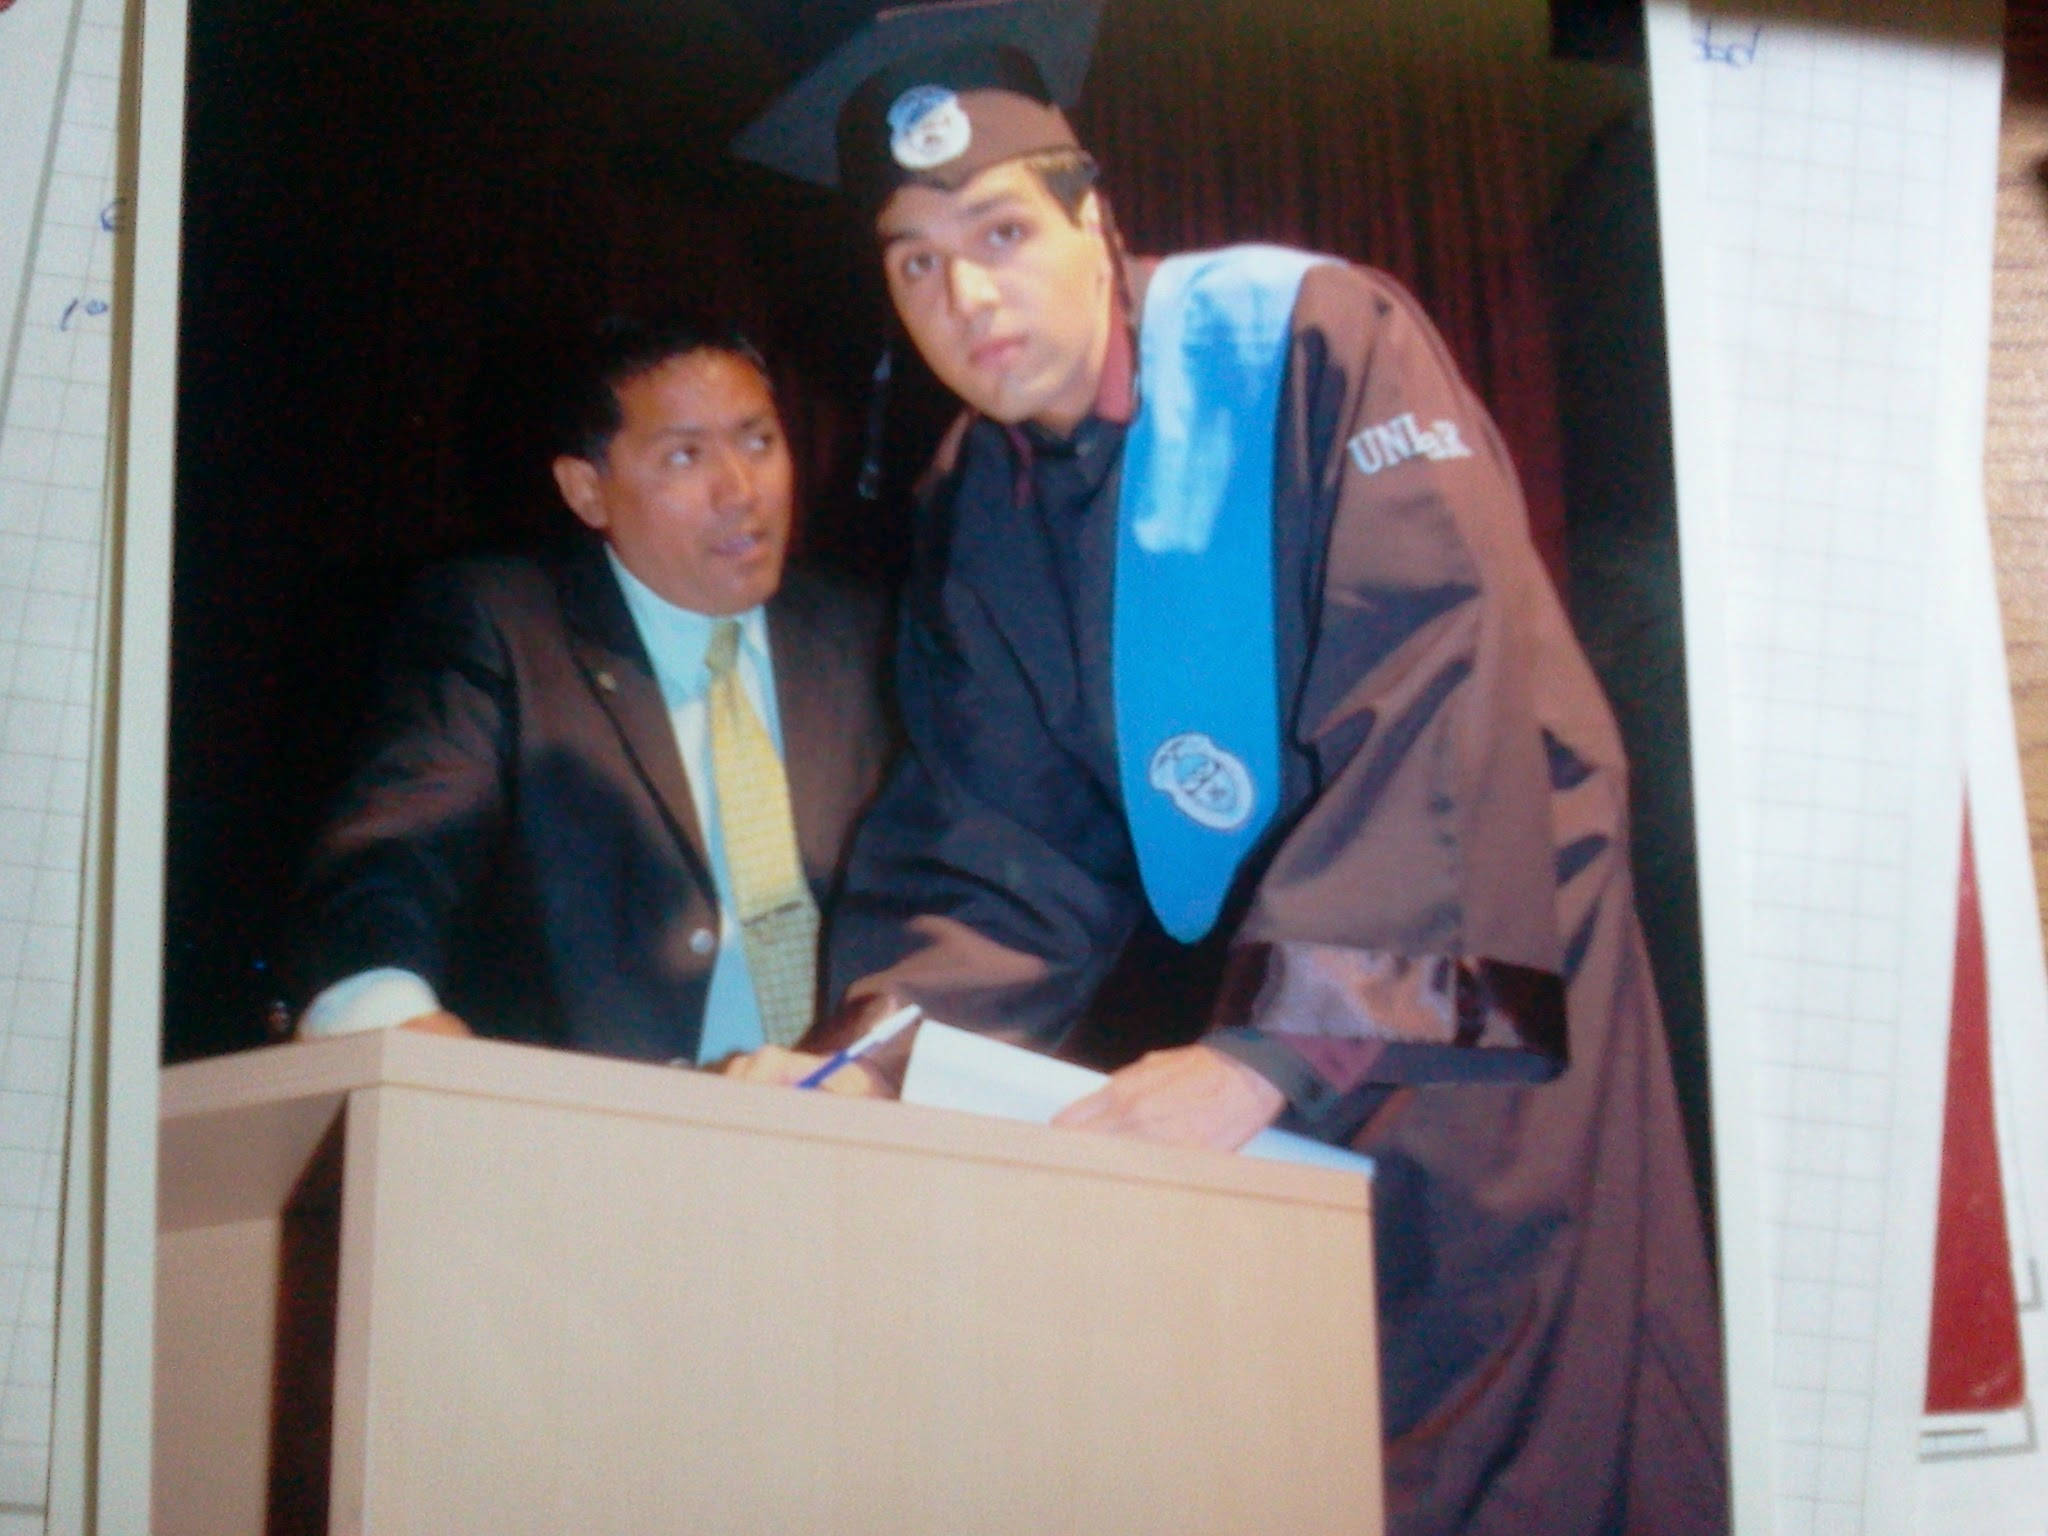
\includegraphics[width=1\linewidth]{images/1}
		\label{fig:UNLAR}
	\end{figure}
\end{frame}

\begin{frame}
	\begin{figure}
		\centering
		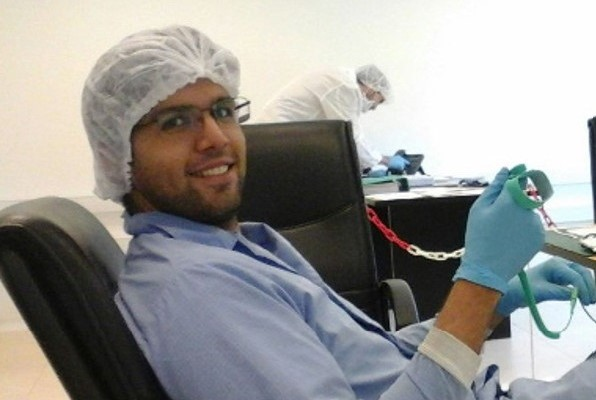
\includegraphics[width=1\linewidth]{images/1.2}
		\label{fig:UNLAR}
	\end{figure}
\end{frame}

\begin{frame}
	\begin{figure}
		\centering
		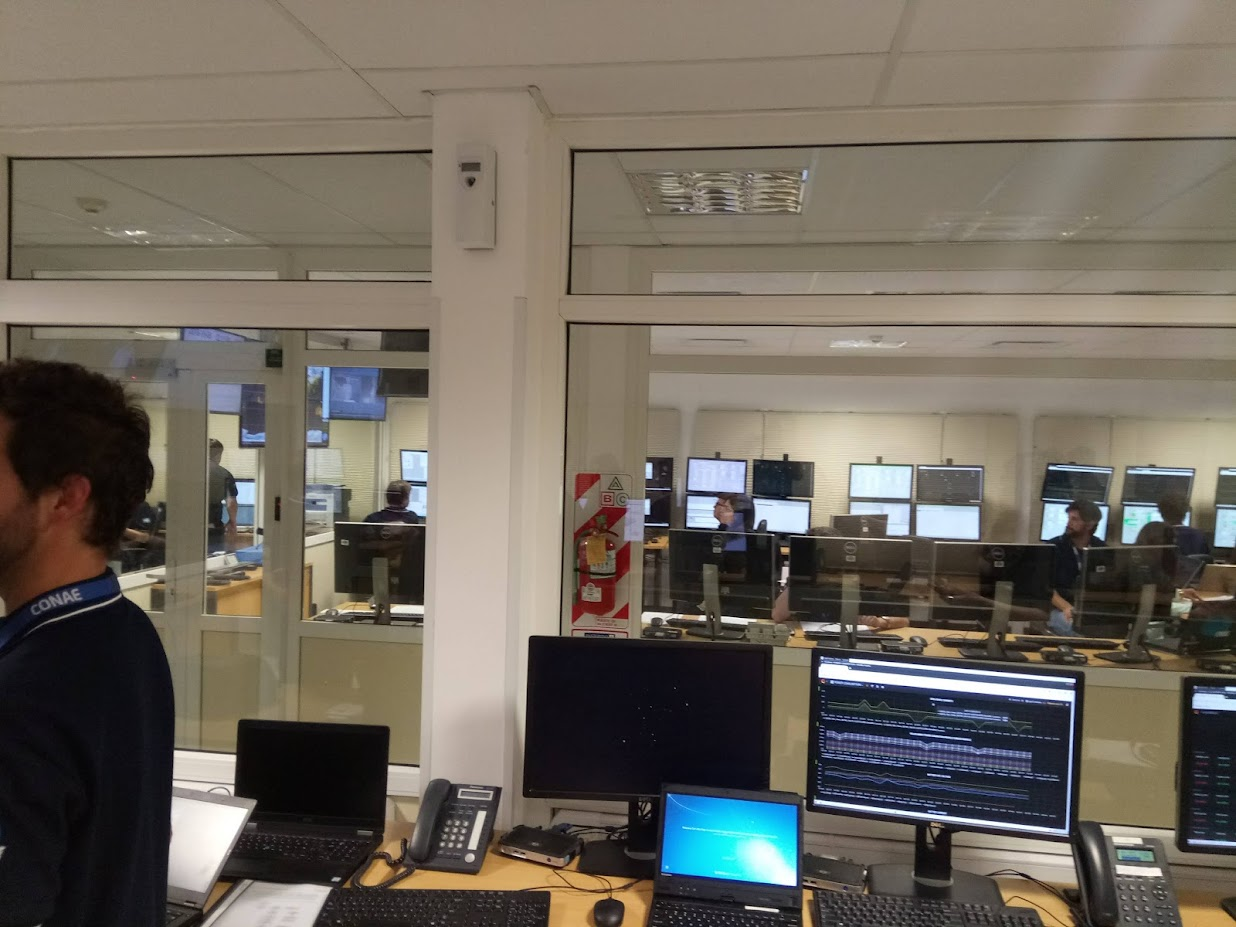
\includegraphics[width=1\linewidth]{images/2}
		\label{fig:UNLAR}
	\end{figure}
\end{frame}

\begin{frame}
	\begin{figure}
		\centering
		
\includegraphics[width=1\linewidth]{images/onapsis}
		\label{fig:UNLAR}
	\end{figure}
\end{frame}

\begin{frame}
  \frametitle {Usuario de Linux desde 2015}
	\begin{figure}
		\centering
		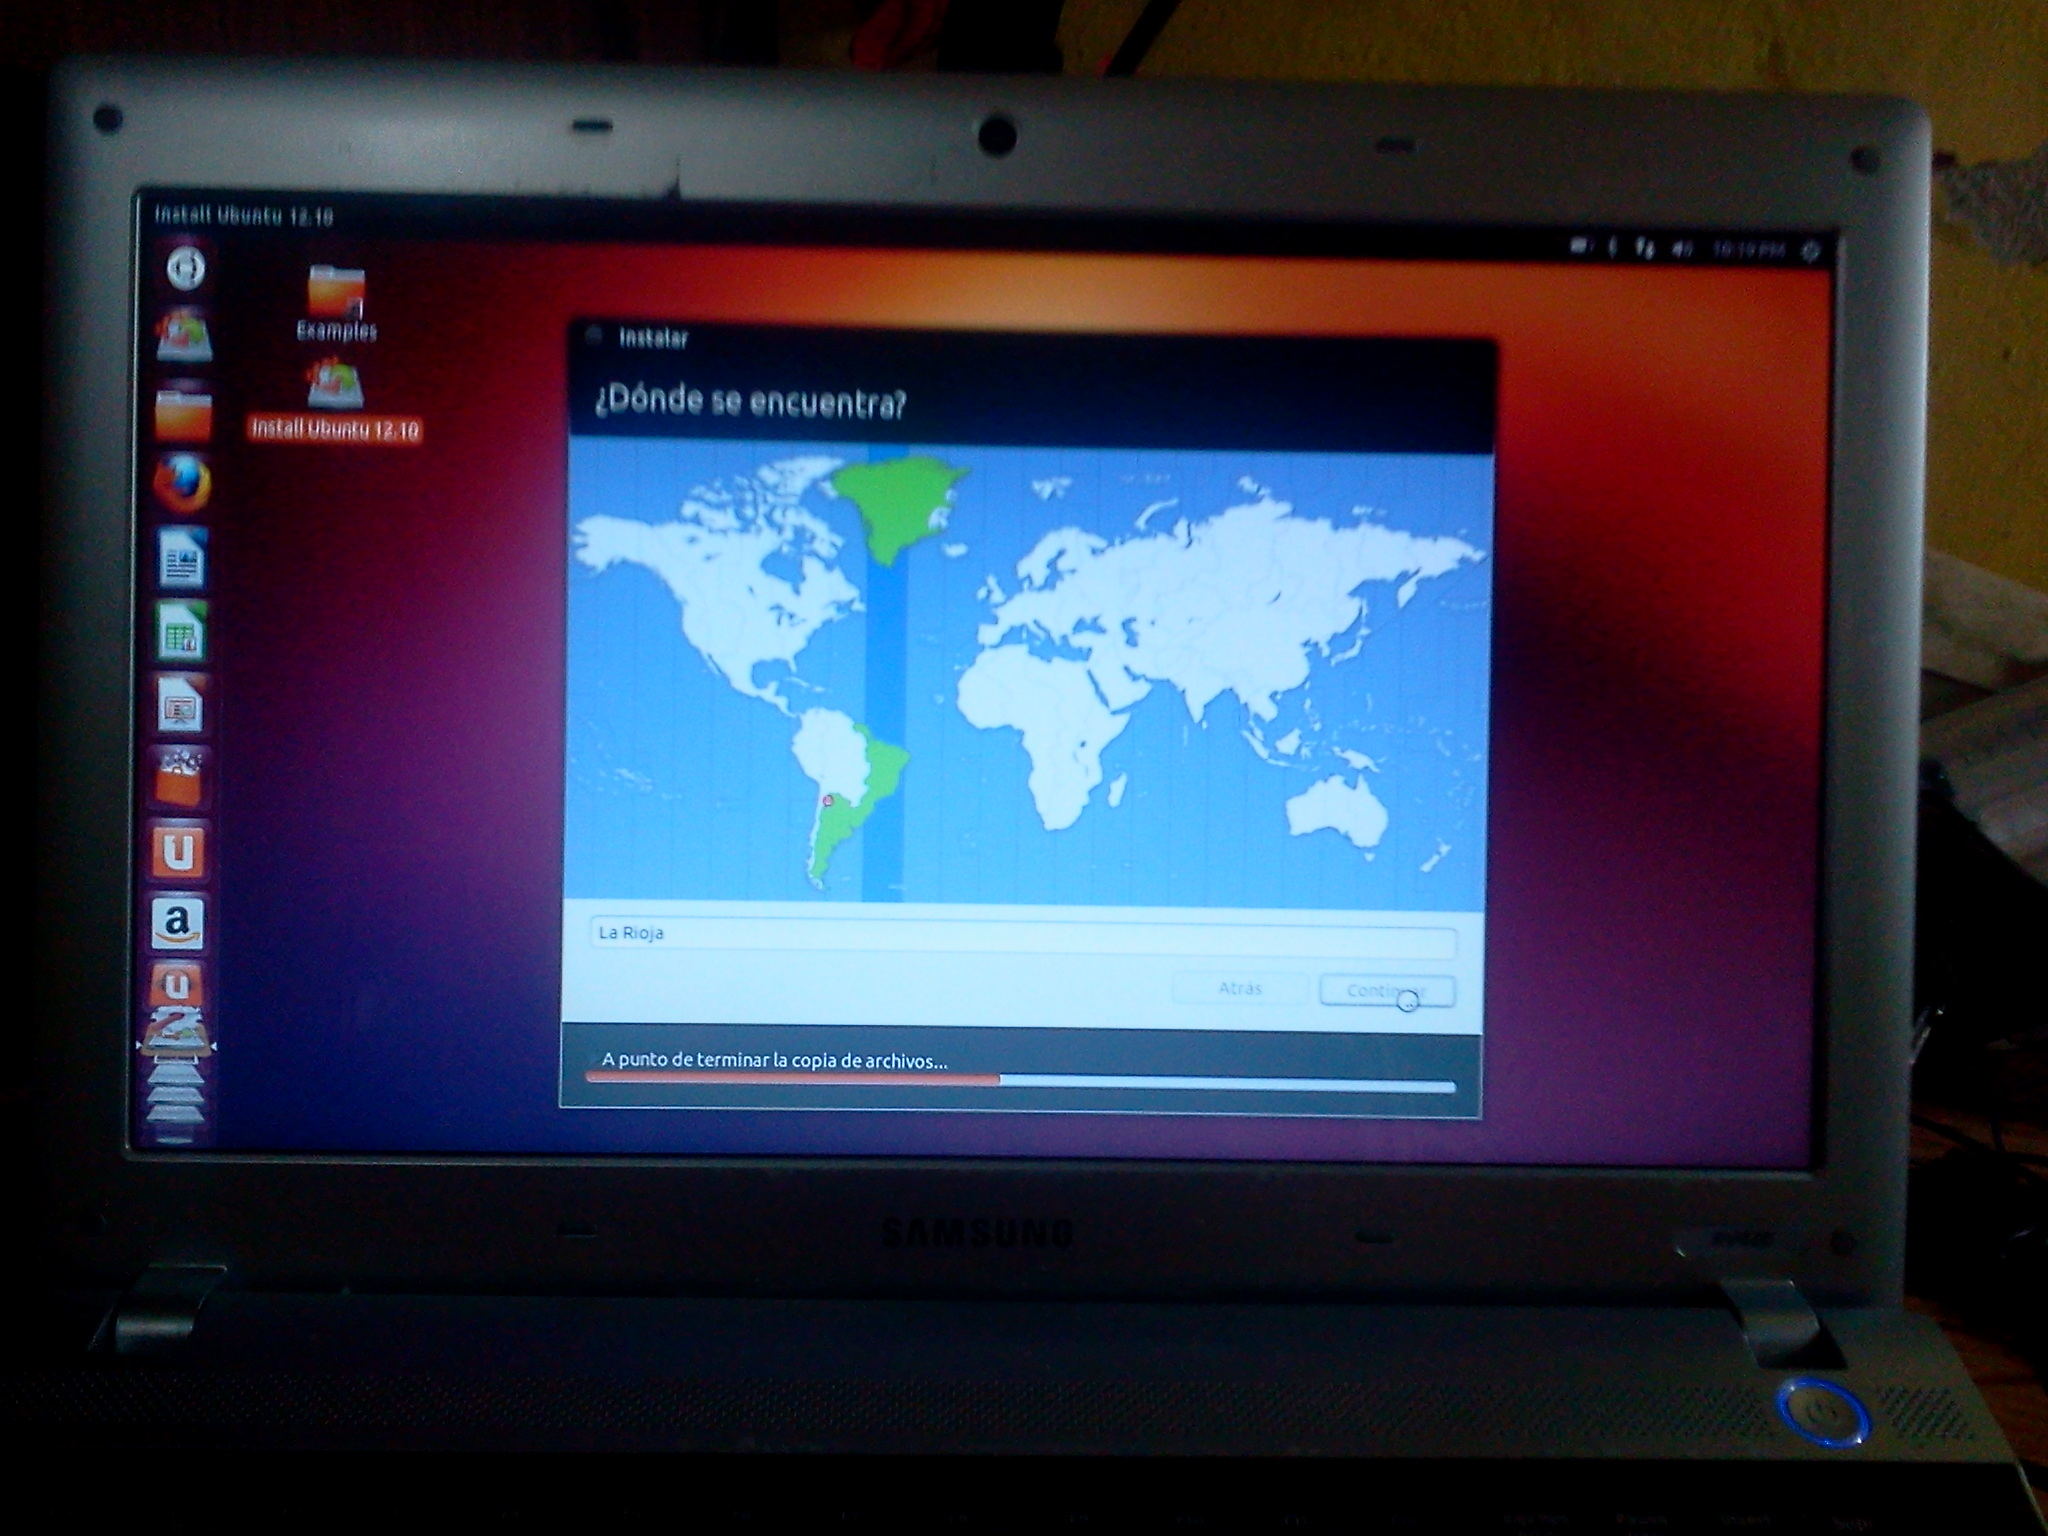
\includegraphics[width=1\linewidth]{images/ubuntu.jpg}
		\label{fig:Ubuntu}
	\end{figure}
\end{frame}

\begin{frame}
  \centering
    \Huge Debian Developer, desde 2023.
\end{frame}

\begin{frame}
  \frametitle {Objetivo}
  \centering
    \Huge Seamos más miembros de Debian en Argentina!!!
\end{frame}

\begin{frame}
    \frametitle {Argentinos en Debian}
    \begin{itemize}
    	\item Agustin Henze
    	\item Marcela Tiznado
    	\item Lisandro Damián Nicanor Pérez Meyer *
    	\item Ulises Vitulli *
    	\item Jose Luis Rivas Contreras
    	\item Emmanuel Arias *
    \end{itemize}

    \vspace{1cm} \\
    \tiny Fuente: https://db.debian.org/
\end{frame}


\begin{frame}
  \frametitle{Argentinos en Debian}
  \centering
  \Huge 1 DD por cada 7.705.805
  \vspace{1cm} \\
  \tiny Fuente: https://www.argentina.gob.ar/pais/poblacion
\end{frame}

\begin{frame}
  \frametitle{Argentinos en Debian}
  \centering
  \Huge 1 DD por cada 915  (Si es que solo hay 5490 del área de sistema en
  Argentina)
  \vspace{1cm} \\
  \tiny Fuente: https://sueldos.openqube.io/encuesta-sueldos-2024.01/
\end{frame}

\begin{frame}
  \frametitle{¿Qué es Debian?}
	\begin{figure}
		\centering
		
\includegraphics[width=0.5\linewidth]{images/debian}
		\label{fig:debian}
	\end{figure}
\end{frame}

\begin{frame}
  \centering
    \Huge Debian es Software libre\\
    \tiny (Libre en el buen sentido de la palabra ;-)
\end{frame}

\begin{frame}{Las 4 Libertades del Software Libre}
  \begin{itemize}
    \item Libertad 0: Ejecutar el software con cualquier propósito \pause
    \item Libertad 1: Estudiar como funciona un programa de software y
      modificarlo segun sus necesidades. \pause
    \item Libertad 2: Redistribuir copias para ayudar a otros \pause
    \item Libertad 3: Distribuir versiones modificada, de modo que toda la
      comunidad se beneficie.
  \end{itemize}
\end{frame}

\begin{frame}
  \centering
    \Huge ¿Qué tan dificil será contribuir a un proyecto de Software libre?
\end{frame}

\begin{frame}
	\begin{figure}
		\centering
		
\includegraphics[width=1\linewidth]{images/hackers.jpg}
		\label{fig:debian}
	\end{figure}
\end{frame}
\begin{frame}
	\begin{figure}
		\centering
		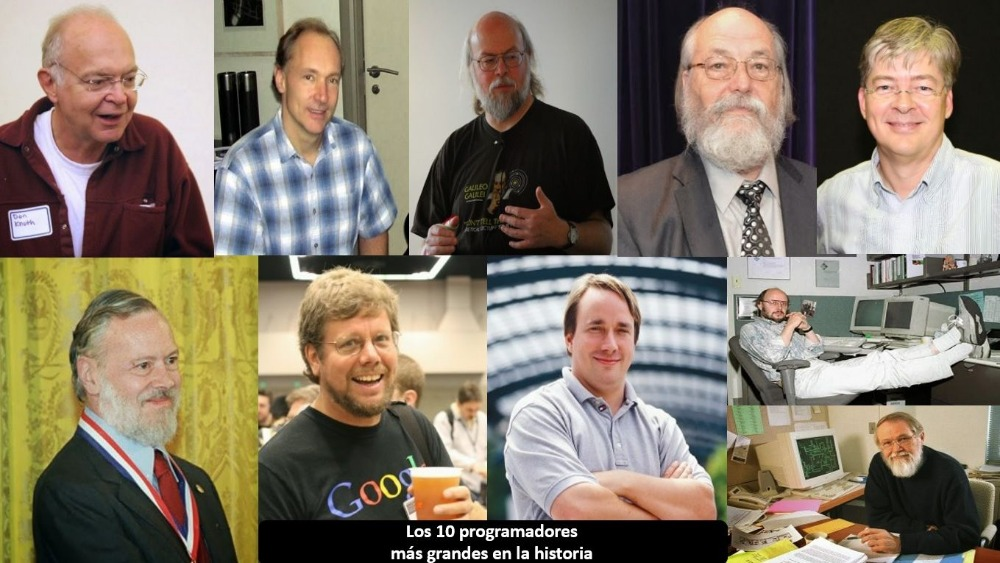
\includegraphics[width=1\linewidth]{images/coders.jpg}
		\label{fig:debian}
	\end{figure}
\end{frame}

\begin{frame}
	\begin{figure}
		\centering
		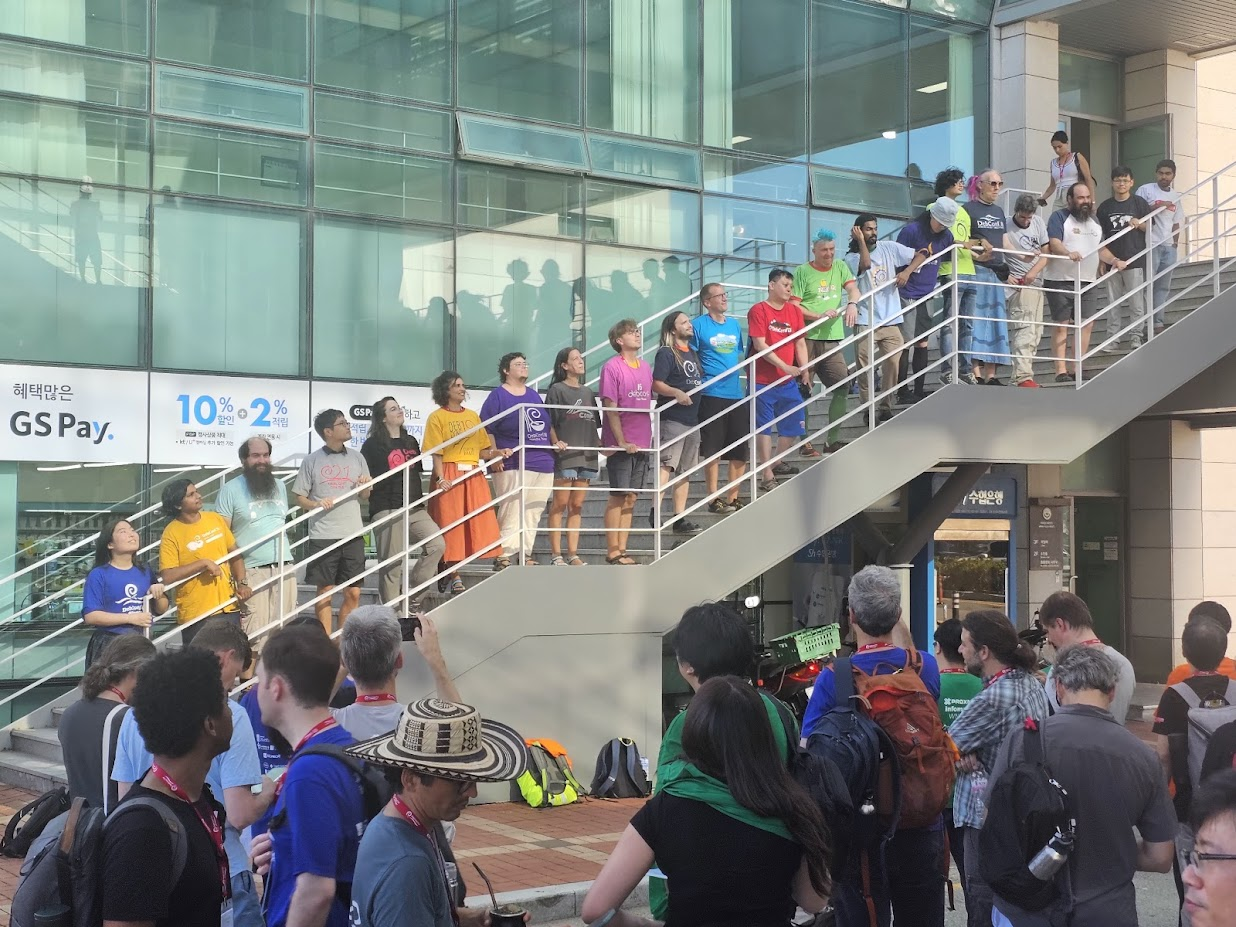
\includegraphics[width=1\linewidth]{images/comunidad.jpg}
		\label{fig:debian}
	\end{figure}
\end{frame}


\begin{frame}
	\begin{figure}
		\centering
		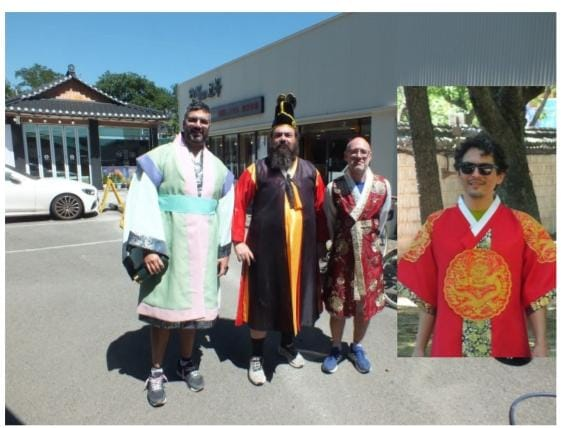
\includegraphics[width=1\linewidth]{images/developers.jpeg}
		\label{fig:debian}
	\end{figure}
\end{frame}

\begin{frame}
	\begin{figure}
		\centering
		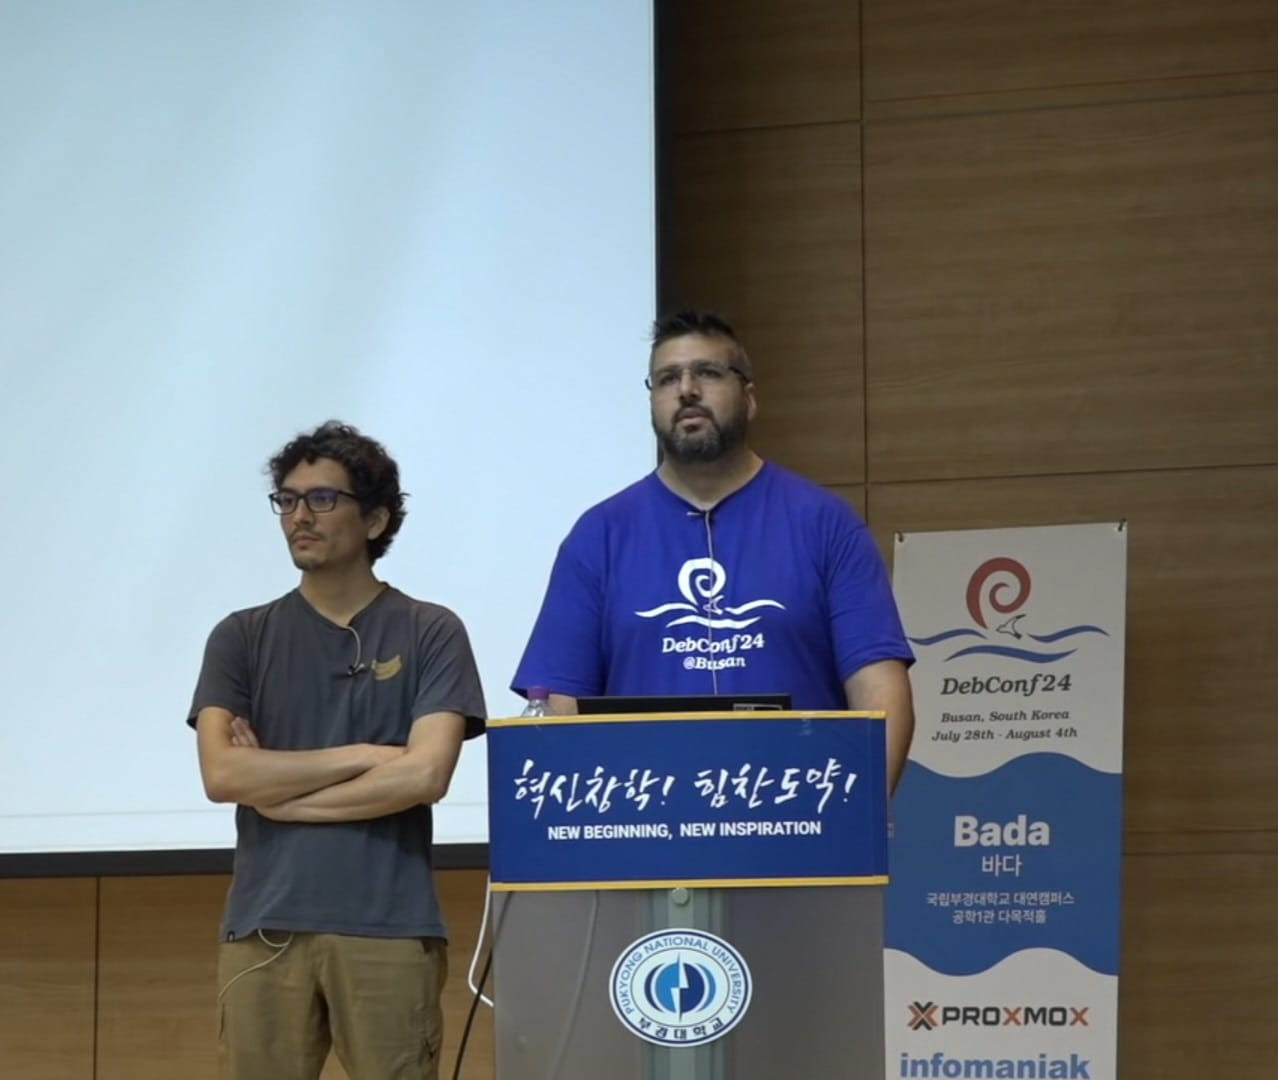
\includegraphics[width=1\linewidth]{images/charla_debian.jpeg}
		\label{fig:debian}
	\end{figure}
\end{frame}

\begin{frame}%[allowframebreaks]
  \frametitle{¿Por qué contribuir a Debian?}
  \begin{itemize}
    \item A algunas personas, sencillamente, les gusta ayudar a los demás, y
      contribuir a un proyecto de software libre es una magnífica manera de
      hacerlo. \pause
    \item Muchos desarrolladores y desarrolladoras escriben programas para
      aprender más acerca de las computadoras, de las diferentes arquitecturas y
      de los lenguajes de programación. \pause
    \item Algunos desarrolladores contribuyen para decir ``''gracias'' por todo
      el excelente software libre que han recibido de otros. \pause
    \item Muchas personas en las instituciones académicas crean software libre
      para compartir el resultado de sus investigaciones. \pause
    \item Las empresas también ayudan a mantener software libre para influir en
      el desarrollo de aplicaciones o para implementar funcionalidades nuevas
      rápidamente. \pause
    \item Desde luego, ¡la mayoría de los desarrolladores de Debian participan
      porque les parece muy divertido!
  \end{itemize}
\end{frame}

\begin{frame}
 \centering
 \Huge Ok, ¿pero como empiezo?
\end{frame}

\begin{frame}
  \centering
  \Huge Usando Debian, hablando de Debian (o cualquier Software Libre)
\end{frame}

\begin{frame}
  \centering
  \Huge Buscando personas que le guste Debian (o el software libre)
\end{frame}

\begin{frame}
  \frametitle {¿Qué tareas puedo realizar?}
  \begin{itemize}
    \item Coding and Maintaining Packages \pause
    \item Testing and Bug Squashing \pause
    \item Writing Documentation and Tagging Packages \pause
    \item Translating and Localizing \pause
    \item Helping other Users \pause
    \item Organizing Events \pause
    \item Use Debian and talk about it
  \end{itemize}
\end{frame}

\begin{frame}
  \centering
  \huge Ultimo Consejo: paciencia, paciencia, paciencia.
\end{frame}

\begin{frame}
  \centering
  \Huge Gracias!!!
\end{frame}

\end{document}
